\section{Project context} 
    The work conducted in this thesis focuses on processing hyperspectral images. This chapter explains in detail what they are and the two most widespread processing methods. 
\section{Hyperspectral Images}
     \subsection{Description}
   Hyperspectral images are defined as an image that has high spectral as well as spatial resolution, which means that a pixel does not have only the 3 colors of reflectance's values characteristic as usual images, they provide spectral information in the whole spectrum instead. HI aims at identifying and estimating the distribution of materials within a captured scene based on their spectral signatures, which represent the normalized measured surface reflectance at each spectral band \cite{manolakis2002detection}.
   
   HI collects high resolution spectral information gathering hundreds of bands from the ultraviolet to the infra-red range of the electromagnetic spectrum. This information is used to distinguish among the different materials composing the captured scene \cite{lee1987synchronous}.
   
   As a first approach, this technology was mostly used for remote sensing applications, however, nowadays it has been widespread among several fields such as medicine, security, agriculture, mineralogy...
   
    On top of that, there is a emerging and rising research linked to three different systems: in-vitro,ex-vivo and in-vivo experiments, the difference among them is the way in which the image has been captured, that is, from a removed tumour or directly from the patient.

    
     \begin{figure}[H]
        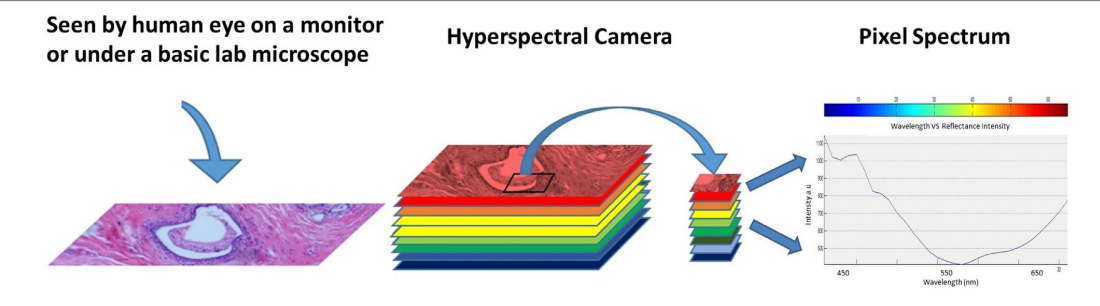
\includegraphics[scale=0.5]{HSI.png}        
        \centering    
        \caption{Hyperspectral image}
        \label{fig:systemArch}
    \end{figure}
       
  
    
  This electromagnetic radiation is not only present among the visible range of wavelengths, as it covers the most part of the electromagnetic spectrum. These kinds of images provide us with useful information as said earlier, as it includes electromagnetic spectrum invisibly to the human eye. However, due to the huge amount of data, processing of HSI images is very computationally expensive.
  
  The experiments of this thesis have been tested using a medical hyperspectral image gathered from the HELICoiD project database. The first illustration displays a dataset of each hyperspectral cube of the brain cancer in RGB,and the second one illustrates the name of each image belonging to the dataset along with their dimensions (rows,columns and bands).
  
  
   \begin{figure}[H]
        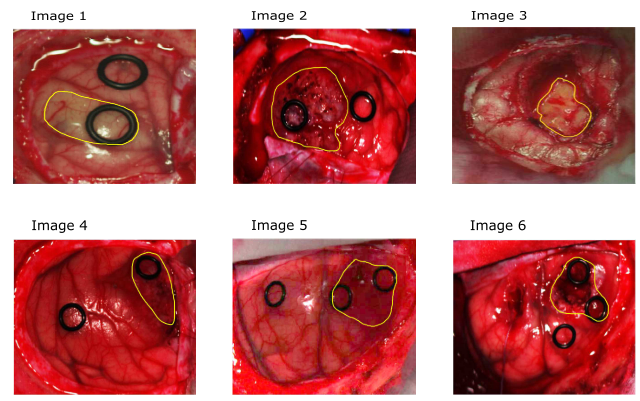
\includegraphics[scale=0.8]{HS_dataset.png}        
        \centering    
        \caption{Brain Cancer dataset}
        \label{fig:systemArch}
    \end{figure}
    
    
   \begin{figure}[H]
        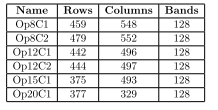
\includegraphics[scale=1.3]{table_dimensions.png}        
        \centering    
        \caption{Dimensions of each image}
        \label{fig:systemArch}
    \end{figure}
     
   \subsection{Applications} 
    Hyperspectral images are mostly used for identifying and estimating different materials within a captured image in the spectral region.
    This technology was initially employed to remote sensing applications, specifically, earth observation and geology. Other than the previously mentioned applications, remote sensing is used in a great variety of applications, such as security and defence, agriculture and food engineering, eye care, mineralogy, surveillance, astronomy... 
    
    
   \subsubsection{Remote Sensing} 

As was mentioned earlier, hyperspectral images are one of the promising remote sensing technology. 

  \subsubsection{Cancer Detection} 

Hyperspectral imaging is a non-contact, non-ionizing and minimally-invasive sensing technique suitable for medicine. It consists in collecting and processing information from across the electromagnetic spectrum creating a hyperspectral image. This kind of images increases the information acquired from a scene compared with a conventional RGB image
Hyperspectral        	
         	
\section{Classifiers}
     
     \subsection{Concept}
      
Image processing consists of a mathematical algorithm that, when applied, derives information from an image that can be used in automated image analysis systems.\cite{khouj2018hyperspectral}. 
 
 	In this context this mathematical algorithm is known as a classifier. The main aim of a classifier is to be able to provide a classification algorithm using observations or data and to train this algorithm based on those data,to finally distinguish at which class belong to.
 
	The process of learning begins with observations or data, such as examples, direct experience, or instruction, in order to look for patterns in data and make better decisions in the future based on the examples that we provide.[pagina web 1] Once the classifier has been trained, it is able to associate any data to a specific class using new input parameters called test dataset. In other words, a classifier is an algorithm that associates the input data to a specific category.
	
	
	The main practical objectives of machine learning consist of generating accurate predictions for unseen items and of designing efficient and robust algorithms to produce these predictions, even for large-scale problems.
	
	
	  \begin{figure}[H]
        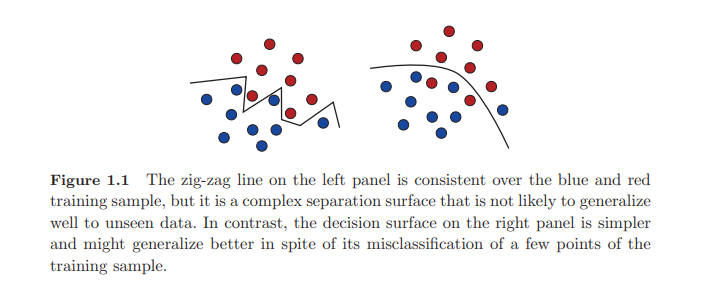
\includegraphics[scale=0.8]{machinelearning.png}        
        \centering    
        \label{fig:systemArch}
    \end{figure}
    
     \subsection{Unsupervised classification}
            
   Input data is not labelled and does not have a known result.

	A model is prepared by deducing structures present in the input data. This may be to extract general rules. It may be through a mathematical process to systematically reduce redundancy, or it may be to organize data by similarity.

	The learner exclusively receives unlabeled training data,and makes predictions for all unseen points. Since in general no labeled example is available in that setting, it can be difficult to quantitatively evaluate the performance of a learner. Clustering and dimensionality reduction are example of unsupervised learning problem\cite{mohri2012foundations}.
	Clustering in its elemental form is defined as a algorithm of identifying homogeneous groups of data points in a given data set.
	The algorithm under study in this master thesis belongs to this kind of classification. This algorithm will be explained in detail later.

    \subsubsection{KMeans} 
                   
K-Means is a learning algorithm used mainly to resolve unsupervised data classification problems. The K-Means algorithm determines k number of centers (one for each cluster),then associate each data point to the nearest centre. 

	It is necessary to define some crucial concepts in order to truly understand this algorithm. A centroid is a data point at the center of a group and each of these groups is called a cluster and is a region in which the density of objects is locally greater than in other zones and share similar features.

	Placing the centroids as far away from each other as can be, when the k centroids are initialized, is the best way of increasing the detection accuracy and minimize the numbers of errors.

 	Furthermore,unsupervised clustering is used to describe processes where a classifier is assigned a dataset without preexisting labels\cite{thomas2002randomized} \cite{kushi2012american}.
 	            
    \subsection{Supervised classification}
            	
The learner receives a set of labeled examples as training data and makes predictions for all unseen points. This is the most common scenario associated with classification, regression, and ranking problems\cite{mohri2012foundations}.

In supervised learning the input data is labeled, which means that each instance of the data set consists of an input vector and a corresponding output value \cite{mohri2012foundations}. A machine learning algorithm solves the problem relying on this label input. The resulting model may be employed for classifying and predicting new unknown data.
	
    \subsection{Processing chain for hyperspectral images}
            
The procedure is as follows; in order to obtain the hyperspectral images of the in- vivo human brain surface during the neurosurgical operations, the HELICoiD project has built a demonstrator capable of simultaneously obtaining two hyperspectral cubes.  

	 A preliminary step called pre-processed is performed in order to decrease the amount of information, such as making a radiometric calibration, reducing the noise and the dimensionality, and finally, normalizing the HS image.Once this preliminary step has been reached, they are analysed using the supervised as well as unsupervised classification.

	In terms of unsupervised classification, HS cubes are clustered employing K-Means, which defines different areas properly, however, they have no meaning. After using this algorithm, an unsupervised segmentation map is generated.Meanwhile in parallel, the system executes a number of algorithms belonging to supervised classification. These algorithms are PCA (Principal Components Analysis), SVM (Support Vector Machine) and KNN (K-Nearest Neighbour). In order to approach real time during surgery, the parallelization of these algorithms is required.

   After performing these algorithms, tissues are displayed using different colours in order to represent the associated classes. 
Applying the majority voting, the unsupervised segmentation map obtained from K-Means clustering algorithm as well as the classification map obtained from supervised classification, are merged. 

	As it can be observed on the image below, the process can be divided into three fundamental parts: the first one belonging to the execution of the PCA and SVM algorithms in parallel. Once it is performed,the process continue with the second part, the implementation of the KNN algorithm. Meanwhile, in parallel with the previous steps (first and second),K-Means is executed.

	  \begin{figure}[H]
        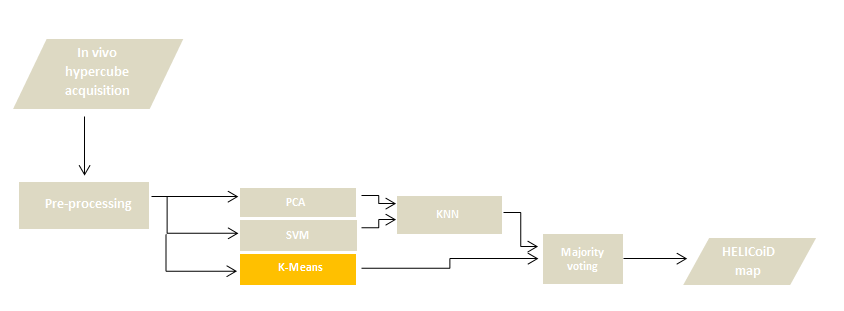
\includegraphics[scale=0.8]{processingchain.png} 
        \caption{HELICoiD processing chain}       
        \centering    
        \label{fig:systemArch}
    \end{figure}
	
	
 	\subsubsection{PCA (Principal Component Analysis)}              
 	\subsubsection{SVN (Support Vector Machine)}
 	\subsubsection{KNN (K-Nearest Neighbor)}

\section{Parameterized and Interfaced Synchronous DataFlow MoC} 
   A wide number of applications within the field of Digital Signal Processing (DSP) such as video decoding, telecommunication and computer vision use Dataflow Models of Computations (MoCs) because of their flexibility, analysability and natural expressivity that ease the parallelization of the applications.
   
   Before going through PiSDF model, we will first define the concept of a Synchronous DataFlow (SDF). SDF is a restricted form of dataflow in which the numbers of tokens produced and consumed by each actor execution are restricted to be constant and statically known (known at compile time)\cite{bhattacharya2001parameterized}.In this kind of model, a graph is used for describing an application in which nodes describe computations and the stream of data-tokens between operations are transmitted by edges. Edges works with initialization tokens called delays as well.
   
   This model called PiSDF extends the semantics of a targeted dataflow MoC and integrates parameterized along with interface-based dataflow. In the case of parameterized dataflow, parameters can have influence on different properties like the firing rules of actors. In the second case,however, predictability is improved since it enables a top-down parametrization and it limits the scope of the parameters. 
   
  Regarding $\pi SDF$ Semantics, a $\pi SDF$ \cite{desnos2013pimm} graph G = (A, F, I, $\Pi$, $\Delta$) contains, in addition to the SDF actor set A and FIFO set F, a set of hierarchical interfaces I, a set of parameters $\Pi$, and a set of parameter dependencies $\Delta$.
   
   \begin{itemize}
   \item Interface-Based Synchronous Dataflow MoC is a hierarchical extension of the SDF model interpreting hierarchy levels as code closures. IBSDF adds interface elements to insulate levels of hierarchy in terms of schedulability analysis \cite{desnos2013pimm}
   
   An example of an IBSDF graph is displayed and explained hereafter:
      
     \begin{figure}[H]
        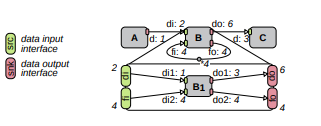
\includegraphics[scale=1]{interfacebsed.png}        
        \centering    
        \caption{Hyperspectral image}
        \label{fig:systemArch}
    \end{figure}
       
A data input interface $i_{data}^{in} \in I_{data}^{in}$ in a subgraph is a vertex transmitting to the subgraph the tokens received by its corresponding data input port. If more tokens are consumed
on a data input interface than the number of tokens received on the corresponding data input port, the data input interface behaves as a circular buffer, producing the same tokens several times.

 A data output interface $i_{data}^{out} \in I_{data}^{out}$ in a subgraph is a vertex transmitting tokens received from the subgraph to its corresponding data output port. If a data output interface
receives too many tokens, it will behave like a circular buffer and output only the last pushed tokens \cite{desnos2013pimm}.

  
   \item Parameterized Dataflow MoCs

Parameterized Dataflow imposes a hierarchy discipline   that incorporates parameterization and run-time management of parameter configurations. Parameters can either be statically defined, or dynamically set by actors at runtime.

As is clearly explained in this paper \cite{bhattacharya2001parameterized},parameterized dataflow modeling framework imposes a hierarchy discipline on an underlying dataflow model and allows subsystem behavior to be controlled by sets of parameters that can be configured dynamically.PSDF can be viewed as an augmentation of the SDF model that comprehensively incorporates parameterization and run-time management of parameter configurations.

\end{itemize}      
         
   \subsection{PREESM} 
      
Nowadays, video coding/decoding or digital communications are applications that are becoming more and more complex and sophisticate. Also, programming architectures such as Digital Signal Processors (DSPs) require high specialization of engineers because of the bottlenecks of the algorithms as well as the architecture, when it comes to implement parallel execution. Therefore, there is a need to implement a more powerful computational models. As was mentioned earlier, the use of parallel architecture may meet requirements.

	To reduce the software development effort for such architectures, it is necessary to provide the programmer with efficient tools capable of automatically solving communications and software partitioning/ scheduling concerns. Most tools such as PeaCE, SynDEx or PREESM use as an entry point a model of the application associated to a model of the architecture\cite{piat2010loop}. The algorithm under study in this work is performed using PREESM.

	PREESM offers great features in terms of memory, time analysis and it has automatic deadlock-free code generation. This tool is an open source rapid prototyping tool. It simulates signal processing applications and generates code for heterogeneous multi/many-core embedded systems. Its dataflow language eases the description of parallel signal processing applications.
	
	Furthermore,PREESM tool inputs are an algorithm graph, an architecture graph, and a scenario which is a set of parameters and constraints that specify the conditions under which the deployment will run. The chosen type of algorithm graph is a parameterized and hierarchical extension of Synchronous Dataflow (SDF) graphs named PiSDF or $\pi SDF$. The architecture graph is named System-Level Architecture Model (S-LAM). From these inputs, PREESM maps and schedules automatically the code over the multiple processing elements and generates multi-core code \cite{pelcat2014preesm}.
	
	
	
	An example of an application graph using PREESM is displayed in figure \ref{fig:graph}.
	
	\begin{figure}[H]
        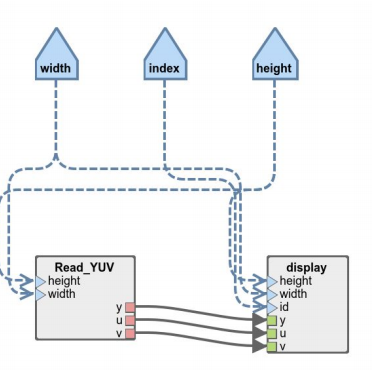
\includegraphics[scale=0.8]{expreesm.png}        
        \centering    
        \caption{Example of application graph \cite{PREESM:2019:Online}}
        \label{fig:graph}
    \end{figure}
	
	This is a typical application graphs that contains the basic components in a network.
	
	Parameters are shown at the upper side, they have impact on the productions and consumption rates of tokens on the data FIFO queues.	
	Actors are entities which are connected each other by First In, First Out data queues (FIFOs). A actor fires when the FIFO have enough incoming tokens. A firing rules set the number of data tokens consumed and produced by an actor.The internal behavior of actors is manually programmed in language supported by the architecture compiler, e.g. C or C++ code.
	
	
	
	
	
	  
  